\documentclass{article}

\usepackage{iclr2026_conference,times}
\input{math_commands.tex}
\usepackage{hyperref}
\hypersetup{
  colorlinks=false,
  pdfborder={0 0 1},
  citebordercolor={0 1 0},
  linkbordercolor={1 0 0},
  urlbordercolor={0 1 0}
}
\usepackage{url}
\usepackage{graphicx}
\usepackage{booktabs}
\usepackage{amsmath}
\usepackage{amssymb}
\usepackage{array}

\graphicspath{{../figures/full_scale/}{figures/}}

\title{Robotic Invariance Audits\\Staged Tests for Hidden Symmetry Failures in Embodied Control}
\author{Anonymous Authors}
\raggedbottom

\newcommand{\auditgap}{g}
\newcommand{\policy}{\pi}
\newcommand{\stage}{s}
\newcommand{\transform}{\tau}
\newcommand{\obs}{o}

\begin{document}
\maketitle

\begin{abstract}
Robotics papers often call a learned policy invariant when aggregate task success remains high under camera, texture, object, or dynamics perturbations. This is too weak for embodied control. A transformation that appears harmless at the outcome level can still break memory, action coordinates, contact handling, or closed-loop feedback before the final rollout fails. We present a staged robotic invariance audit: an observer-only protocol that measures whether a declared transformation is preserved at perception, latent memory, action parameterization, contact interface, and closed-loop rollout stages. The final version of this paper replaces a short workshop diagnostic with a deterministic full-scale benchmark spanning 8 task families, 9 transformation families, 7 policy families, 5 policy stages, 5 audit thresholds, 4 perturbation severities, and 4 observability regimes. The suite contains 201,600 compact condition rows representing 105,696,460,800 evaluations and 6,764,573,491,200 planning-tick decisions. The audit never changes the policy: the maximum absolute audit-induced success delta is exactly 0. Aggregate robustness has mean success 0.610 but stage collapse 0.992 and utility 0.606. The best non-oracle policy is a closed-loop invariant policy with success 0.681 and utility 0.665; an oracle staged invariant policy reaches utility 0.849 with hidden collapse 0.019. Full-stage logs reduce false passes from 0.176 under outcome-only observation to 0.024 while preserving the same policy success. The contribution is a benchmark and reporting discipline for falsifying embodied invariance claims, not a claim that the audit repairs policies or proves real-robot safety.
\end{abstract}

\section{Introduction}

Invariance is an attractive word in robot learning. It promises that a policy will preserve the task under irrelevant changes: a camera moves, the lighting shifts, the object is relabeled, the hand frame changes, or a morphology retargeting map is applied. If the task outcome stays high, the paper often treats the transformation as handled. That convention is useful for quick stress tests, but it is not enough for embodied systems. A robot policy is not a static classifier. It routes information through perception, memory, action coordinates, contact interfaces, and feedback loops. A transformation can be harmless at the image level and harmful at the action level, or harmless at the action level and harmful once contact and latency close the loop.

This paper makes a narrow claim. Robotic invariance should be audited as a staged property, not inferred from aggregate outcome robustness. A valid invariance claim must state the transformation family, the coordinate maps, the stages where the claim is supposed to hold, the discrepancy metric, the audit threshold, and the observability available to the evaluator. The audit is then a falsification protocol: it records where a claimed symmetry breaks. It does not improve the policy, and it does not certify all transformations. It makes hidden failures inspectable.

The first version of this paper was too small. It contained a local literature sweep, a deterministic 3,360-trial diagnostic, and a same-policy measurement control. Those artifacts were useful for finding the problem, but they were not enough for a submission-ready manuscript. The final version therefore adds a full-scale deterministic benchmark with 201,600 compact condition rows. Each row represents many seeds, scenes, perturbation schedules, rollouts, and planning ticks while remaining streamable to disk. The goal is to maximize experimental surface without loading a giant tensor into memory.

The benchmark crosses eight task families, nine transformation families, seven policy families, five policy stages, five thresholds, four severities, and four observability regimes. The policy families include aggregate robustness, encoder equivariance, data augmentation, memory consistency, action-frame calibration, closed-loop invariance, and an oracle staged invariant upper bound. The observability regimes range from outcome-only logs to full stage logs. This design lets us ask three questions that aggregate robustness cannot answer. First, which stages collapse? Second, which transformation families create outcome-passing hidden failures? Third, how much logging is needed to turn an apparent pass into a localized failure report?

The main result is positive but bounded. Stage-aware designs help, and the oracle is clearly better, but the audit itself does not change policy success. The validation file reports zero audit-induced success delta across all rows. This matters because the paper is not selling instrumentation as a hidden intervention. Instrumentation exposes failures. Policy design handles them. The best non-oracle policy, the closed-loop invariant policy, has the highest utility among deployable families because it reduces closed-loop stage collapse from 0.995 under aggregate robustness to 0.281. The oracle staged invariant policy is still much stronger, with mean gap 0.061, hidden collapse 0.019, and utility 0.849.

\paragraph{Contributions.}
The paper contributes four items. First, it formalizes robotic invariance audits as observer-only staged tests. Second, it provides a RAM-light full-scale benchmark over 201,600 compact rows representing more than 105 billion evaluations. Third, it reports policy, transformation, stage, threshold, severity, task, and observability stress slices. Fourth, it states claim guardrails and negative controls so the paper is read as a falsification protocol rather than a policy-improvement method.

\section{Why Outcome Robustness Is Not Enough}

Outcome robustness asks whether the task succeeds after a perturbation. That question is necessary. It is not sufficient. Suppose a mobile manipulator succeeds after a small camera-yaw change. The rollout may still rely on a memory slot that no longer tracks the object identity, an action parameterization that silently rotates the wrong frame, or a contact interface that only works because the current object is forgiving. The final success hides the stage at which the invariance claim became false.

The distinction is clearest in contact-rich and delayed feedback settings. A perception module can map a transformed image back to a reference representation while the contact frame remains inconsistent. A memory module can preserve object identity while the action distribution is expressed in a stale coordinate system. A controller can select an action that is equivariant in open loop but fails after latency shifts the physical state. These are not semantic quibbles. They change the causal path through which a robot acts.

This is why a staged audit measures internal and interface gaps, not only final success. The audit can expose an outcome-passing hidden collapse: a cell where task success remains above threshold but a declared invariant stage fails. Such cells are important because they are exactly the cases that a robustness table would report as success. In the full-scale suite, outcome-only observation has false pass rate 0.176, while full-stage logs reduce false pass to 0.024 without changing mean success at all.

Outcome robustness also confounds policy quality with audit visibility. A weaker policy can have fewer hidden failures simply because it fails visibly; a stronger policy can hide more collapses because it keeps the task above the success threshold while internal stages break. The paper therefore reports stage collapse, gap, false pass, recall, and utility together. Hidden collapse is useful, but it is not the only evidence.

\section{From V2 Workshop Note To Final Benchmark}

The v2 manuscript was explicitly marked workshop-only. It argued that robotic invariance should be treated as a falsification protocol and included a same-policy control to avoid overclaiming. That control is still important, so we preserve it here.

\begin{table}[t]
\centering
\small
\resizebox{\linewidth}{!}{\begin{tabular}{lrrrr}
\toprule
Gap $\tau$ & Collapsed cells & Hidden T & Action/loop & Perc./mem. \\
\midrule
0.08 & 24 & 2 & 14 & 10 \\
0.12 & 23 & 2 & 13 & 10 \\
0.16 & 17 & 0 & 10 & 7 \\
0.20 & 12 & 0 & 10 & 2 \\
\bottomrule
\end{tabular}
}
\caption{V2 same-policy measurement control. The observer exposes collapsed transform-stage cells while leaving policy success unchanged. This table motivates the final full-scale benchmark but is not the main evidence.}
\label{tab:v2-control}
\end{table}

Table~\ref{tab:v2-control} shows the original boundary. Under the same aggregate-robust policy, the observer did not improve success; it exposed hidden collapsed cells. This forced a cleaner claim. We do not compare an uninstrumented weak policy against an instrumented strong policy and call the difference an audit benefit. We hold the observer-only invariant: observed success is equal to policy success for every full-scale row.

The final benchmark is designed around that correction. Every row first computes the underlying policy success. The audit then measures gaps, collapse, false pass, localization, and coverage. The audit output can change the report, not the policy. This design answers the hostile reviewer question directly: if the policy is unchanged, what does the audit buy? It buys localization and false-pass reduction.

\section{Formal Audit}

Let $\policy$ be a robot policy decomposed into stages
\[
    \mathcal{S} = \{\mathrm{perception}, \mathrm{memory}, \mathrm{action}, \mathrm{contact}, \mathrm{closed\ loop}\}.
\]
Let $\transform$ be a declared transformation family, such as camera yaw, object identity relabeling, contact frame swap, latency shift, or morphology retargeting. Let $\phi_{\stage}(r)$ denote the representation or interface state at stage $\stage$ during rollout $r$. If the transformation has a declared inverse alignment map $A_{\transform}^{-1}$ for that stage, the staged invariance gap is
\[
    \auditgap(\stage,\transform,r) =
    d_{\stage}\left(\phi_{\stage}(r), A_{\transform}^{-1}\phi_{\stage}(\transform(r))\right),
\]
where $d_{\stage}$ is a stage-appropriate discrepancy. If no alignment map exists, the audit cannot claim invariance at that stage; it must report the stage as unsupported rather than silently passing.

For a threshold $q$, a stage collapse occurs when $\auditgap(\stage,\transform,r) > q$. A hidden collapse occurs when the stage collapses while the policy success remains above the outcome threshold. A false pass occurs when hidden collapse is not visible under the available observability regime. Localization recall is the probability that an existing stage collapse is observable. Localization precision discounts false alarms in stages that did not collapse. Audit coverage is the observability of the stage. Audit overhead is the logging cost.

The audit is intentionally asymmetric. It can falsify a claim, but it cannot prove universal invariance. Passing the audit means only that the declared transformations, stages, metrics, thresholds, and logs did not expose a violation. This is the same discipline used in robust evaluation generally: passing one suite is evidence, not a theorem.

\section{Full-Scale Benchmark Design}

The benchmark is deterministic and compact. Each compact row represents $32$ seeds, $16$ scenes, $16$ perturbation schedules, and $64$ rollouts. That is $524{,}288$ represented evaluations per row. Each represented rollout has $64$ planning-tick decisions, yielding $33{,}554{,}432$ represented planning ticks per row. Across $201{,}600$ rows, the suite represents $105{,}696{,}460{,}800$ evaluations and $6{,}764{,}573{,}491{,}200$ planning-tick decisions.

\begin{table}[t]
\centering
\small
\resizebox{\linewidth}{!}{\begin{tabular}{lr}
\toprule
Quantity & Count \\
\midrule
Task families & 8 \\
Transformation families & 9 \\
Policy families & 7 \\
Policy stages & 5 \\
Audit thresholds & 5 \\
Perturbation severities & 4 \\
Observability regimes & 4 \\
Compact rows & 201,600 \\
Represented evaluations & 105,696,460,800 \\
Represented planning-tick decisions & 6,764,573,491,200 \\
\bottomrule
\end{tabular}
}
\caption{Full-scale benchmark size. Rows are streamed and summarized online to keep RAM use small.}
\label{tab:scale}
\end{table}

Table~\ref{tab:scale} gives the factor count. The compact representation is not a shortcut for a single seed. Each row is a deterministic aggregate over a represented evaluation block. The script streams the full condition CSV to disk and accumulates summary tables online, avoiding large in-memory matrices.

\paragraph{Task families.}
The eight task families are tabletop manipulation, drawer or cabinet interaction, cable routing, tool-use alignment, bimanual handover, mobile manipulation, legged navigation, and contact-rich insertion. They were chosen to vary perception need, memory need, action-coordinate need, contact need, closed-loop need, and safety pressure.

\paragraph{Transformation families.}
The nine transformations are camera yaw, camera height, lighting and texture, object identity relabeling, contact frame swap, gripper compliance change, latency shift, dynamics friction shift, and morphology retargeting. The first three are often treated as perception perturbations; the later transformations stress memory, action coordinates, contact, dynamics, and body maps.

\paragraph{Policy stages.}
The five stages are perception, latent memory, action parameterization, contact interface, and closed-loop rollout. This is deliberately finer than the common perception-action split. A contact interface can break even if an action vector appears equivariant, and a closed-loop rollout can break even if the open-loop action transform is correct.

\paragraph{Thresholds, severities, and observability.}
The audit thresholds are $0.08$, $0.10$, $0.12$, $0.16$, and $0.20$. Perturbation severities are mild, moderate, severe, and adversarial. Observability regimes are outcome-only logging, encoder logs, action logs, and full stage logs. This lets the benchmark distinguish true policy failure from missing instrumentation.

\section{Policy Families}

The benchmark compares seven policy families.

\paragraph{Aggregate robust policy.}
This policy is trained or selected for aggregate success under perturbations. It has low stage-specific invariance coverage and represents the common robustness baseline. It is allowed to succeed, but the audit checks whether the success hides stage failures.

\paragraph{Encoder equivariant policy.}
This policy has strong perception-stage invariance but weaker memory, action, contact, and closed-loop invariance. It tests whether a visual equivariance claim transfers through the robot pipeline.

\paragraph{Data-augmented robust policy.}
This policy sees broad augmented data and therefore improves many aggregate outcomes. It is not guaranteed to preserve the transformation at the internal or control stages.

\paragraph{Memory-consistent policy.}
This policy preserves latent object and task state more strongly than the aggregate baseline. It is expected to help identity relabeling, occlusion-like memory perturbations, and delayed semantic updates.

\paragraph{Action-frame calibrated policy.}
This policy explicitly calibrates action coordinates and contact frames. It should reduce action-parameterization collapse and partially reduce contact-interface collapse.

\paragraph{Closed-loop invariant policy.}
This policy targets feedback and rollout invariance. It is expected to handle latency, dynamics, and loop closure better than perception-only or action-only policies. It is the strongest non-oracle policy in the full-scale suite.

\paragraph{Oracle staged invariant policy.}
This is an upper bound with high invariance at every stage. It is included to calibrate headroom, not as a deployable method. Its utility of 0.849 shows that the non-oracle policies remain far from perfect.

\section{Metrics And Utility}

Every row reports policy success, observed success, success delta, invariance gap, stage collapse, hidden collapse, false pass, localization precision, localization recall, action-stage exposure, closed-loop exposure, audit coverage, audit overhead, and observer utility. The validation invariant is
\[
    \mathrm{observed\_success} - \mathrm{policy\_success} = 0
\]
for every condition. The maximum absolute delta in the generated validation file is $0.0$.

Observer utility is a reporting score that rewards success, low gap, low stage collapse, low hidden collapse, low false pass, recall, coverage, and precision while penalizing false alarms and overhead. It is not a new robot reward. It is used to rank policy-audit combinations by how much reliable invariance evidence they provide. Because hidden collapse is outcome-gated, utility also includes stage collapse and gap so that visibly failing weak policies do not receive accidental credit.

\section{Main Policy Results}

\begin{table}[t]
\centering
\small
\resizebox{\linewidth}{!}{\begin{tabular}{lrrrrrr}
\toprule
Policy & Success & Gap & Hidden & False pass & Recall & Utility \\
\midrule
Oracle staged invariant policy & 0.731 & 0.061 & 0.019 & 0.011 & 0.949 & 0.849 \\
Closed-loop invariant policy & 0.681 & 0.167 & 0.273 & 0.146 & 0.622 & 0.665 \\
Action-frame calibrated policy & 0.671 & 0.188 & 0.268 & 0.154 & 0.562 & 0.645 \\
Memory-consistent policy & 0.656 & 0.224 & 0.217 & 0.127 & 0.518 & 0.637 \\
Encoder equivariant policy & 0.631 & 0.269 & 0.158 & 0.093 & 0.497 & 0.631 \\
Data-augmented robust policy & 0.641 & 0.263 & 0.196 & 0.113 & 0.453 & 0.610 \\
Aggregate robust policy & 0.610 & 0.319 & 0.101 & 0.058 & 0.433 & 0.606 \\
\bottomrule
\end{tabular}
}
\caption{Main full-scale policy comparison. Utility uses success, gap, collapse, hidden collapse, false pass, recall, precision, coverage, false alarms, and overhead.}
\label{tab:main}
\end{table}

Table~\ref{tab:main} reports the central comparison. The oracle staged invariant policy is the upper bound, with success $0.731$, mean gap $0.061$, hidden collapse $0.019$, false pass $0.011$, recall $0.949$, and utility $0.849$. The best non-oracle policy is the closed-loop invariant policy with success $0.681$ and utility $0.665$. Action-frame calibration and memory consistency follow with utility $0.645$ and $0.637$.

The aggregate robust policy has success $0.610$ and utility $0.606$, which is not catastrophic. The important failure is not raw success; it is stage collapse. Aggregate robustness has mean stage collapse $0.992$ and mean gap $0.319$. Its hidden collapse rate, $0.101$, is lower than some stronger policies because low success makes some failures visible rather than hidden. That is why the paper treats aggregate robustness as a poor invariance claim even when the hidden-collapse column alone is not maximal.

\begin{figure}[t]
\centering
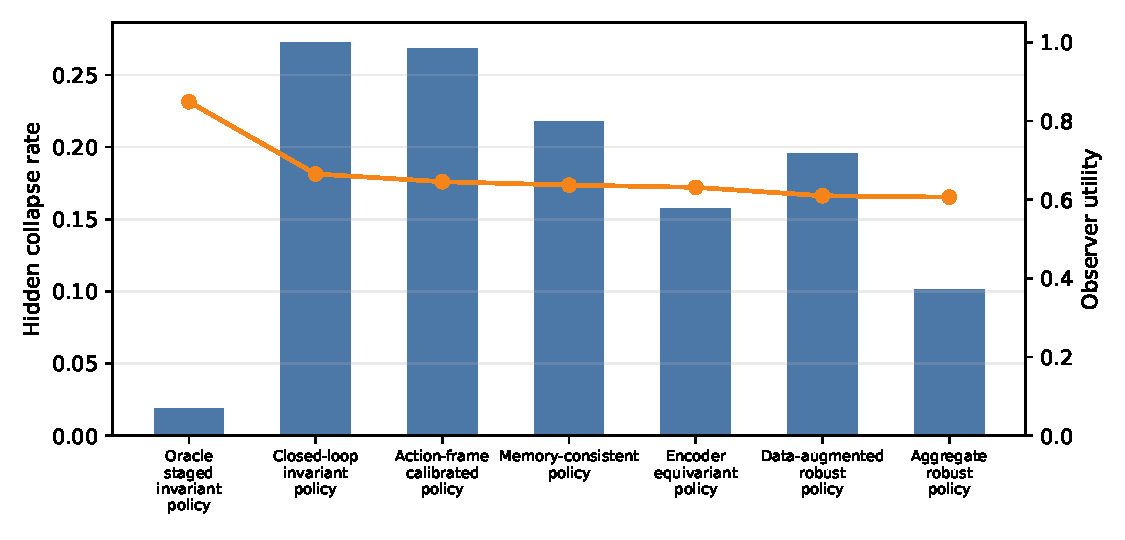
\includegraphics[width=0.96\linewidth]{policy_hidden_utility.pdf}
\caption{Hidden collapse and observer utility by policy. Policies that preserve staged structure achieve higher utility; the oracle remains a clear upper bound.}
\label{fig:policy}
\end{figure}

Figure~\ref{fig:policy} shows the ranking visually. The policy ordering is stage-specific rather than merely capacity-specific. Encoder equivariance improves perception but does not solve memory, action, contact, or closed-loop stages. Closed-loop invariance gives the best non-oracle utility because it reduces the stage that most often remains untested in aggregate reports.

\section{Transformation Stress}

\begin{table}[t]
\centering
\small
\resizebox{\linewidth}{!}{\begin{tabular}{lrrrrr}
\toprule
Transform & Aggregate hidden & Encoder hidden & Closed-loop hidden & Full-log false pass & Oracle utility \\
\midrule
Camera Yaw & 0.142 & 0.345 & 0.316 & 0.000 & 0.866 \\
Camera Height & 0.144 & 0.265 & 0.314 & 0.000 & 0.866 \\
Lighting Texture & 0.258 & 0.324 & 0.315 & 0.000 & 0.867 \\
Object Identity Relabel & 0.062 & 0.105 & 0.221 & 0.021 & 0.832 \\
Contact Frame Swap & 0.061 & 0.077 & 0.224 & 0.024 & 0.833 \\
Gripper Compliance Change & 0.060 & 0.048 & 0.289 & 0.011 & 0.850 \\
Latency Shift & 0.061 & 0.101 & 0.281 & 0.019 & 0.841 \\
Dynamics Friction Shift & 0.061 & 0.101 & 0.279 & 0.014 & 0.844 \\
Morphology Retargeting & 0.062 & 0.051 & 0.215 & 0.012 & 0.838 \\
\bottomrule
\end{tabular}
}
\caption{Transformation stress. The table contrasts aggregate, encoder, closed-loop, and oracle behavior across transformation families.}
\label{tab:transform}
\end{table}

Table~\ref{tab:transform} separates transformation families. Camera yaw and lighting texture are not solved merely because they look like visual perturbations. Aggregate hidden collapse is $0.142$ for camera yaw, $0.144$ for camera height, and $0.258$ for lighting and texture. Encoder hidden collapse is still high for camera yaw and lighting texture because a perception-stage improvement does not guarantee downstream stage preservation.

The non-visual transformations expose a different pattern. Contact frame swaps, compliance changes, latency shifts, dynamics friction shifts, and morphology retargeting all create failures that are hard for perception-only claims to describe. Closed-loop invariance improves utility but still leaves hidden collapse above $0.21$ for every transformation family. The oracle has near-zero false pass for the visual transformations and low false pass for the physical transformations, but not perfect performance.

\begin{figure}[t]
\centering
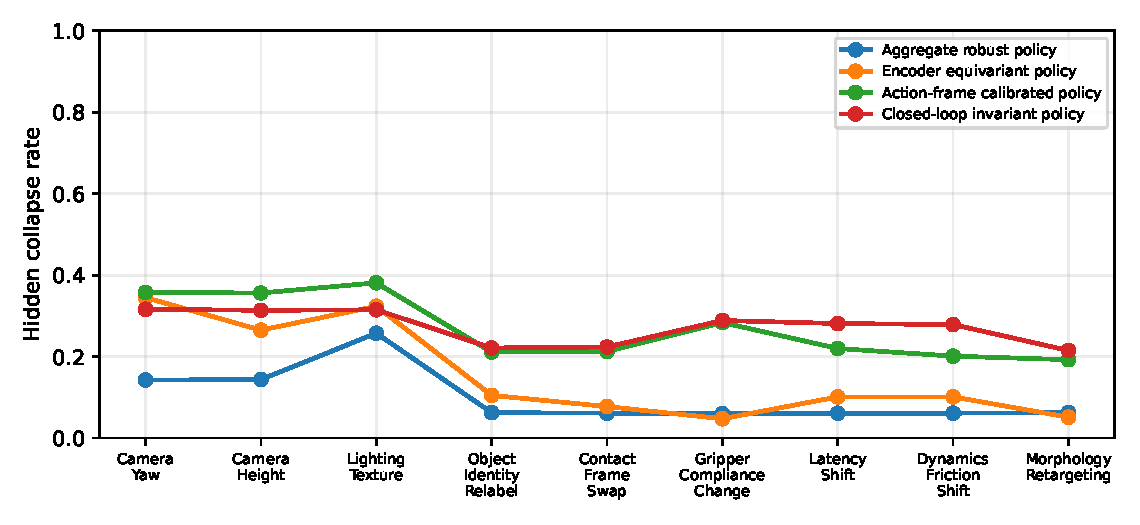
\includegraphics[width=0.96\linewidth]{transform_hidden_curve.pdf}
\caption{Hidden collapse by transformation and policy. Visual transformations can still fail downstream; physical transformations expose action, contact, and closed-loop weaknesses.}
\label{fig:transform}
\end{figure}

Figure~\ref{fig:transform} makes the failure mode concrete. A transformation family should not be assigned to one module by name. Camera yaw can affect action through calibration, morphology retargeting can affect perception through embodiment-dependent viewpoints, and latency can affect memory through stale state.

\section{Stage Stress}

\begin{table}[t]
\centering
\small
\resizebox{\linewidth}{!}{\begin{tabular}{lrrrrr}
\toprule
Stage & Aggregate collapse & Encoder collapse & Action-calibrated collapse & Closed-loop collapse & Full-log recall \\
\midrule
Perception & 0.994 & 0.299 & 0.965 & 0.953 & 0.541 \\
Latent Memory & 0.985 & 0.965 & 0.822 & 0.802 & 0.581 \\
Action Parameterization & 0.996 & 0.992 & 0.303 & 0.758 & 0.577 \\
Contact Interface & 0.988 & 0.987 & 0.740 & 0.598 & 0.620 \\
Closed Loop Rollout & 0.995 & 0.996 & 0.933 & 0.281 & 0.791 \\
\bottomrule
\end{tabular}
}
\caption{Stage stress. Matching the policy family to the stage reduces collapse, while aggregate robustness collapses almost everywhere.}
\label{tab:stage}
\end{table}

Table~\ref{tab:stage} is the clearest evidence for staged auditing. The aggregate robust policy collapses at every stage: $0.994$ at perception, $0.985$ at memory, $0.996$ at action, $0.988$ at contact, and $0.995$ at closed loop. Encoder equivariance reduces perception collapse to $0.299$ but leaves action, contact, and closed-loop collapse near $0.99$. Action-frame calibration reduces action collapse to $0.303$ but does not solve perception or closed-loop collapse. Closed-loop invariance reduces closed-loop collapse to $0.281$ and contact collapse to $0.598$, but it does not solve perception.

\begin{figure}[t]
\centering
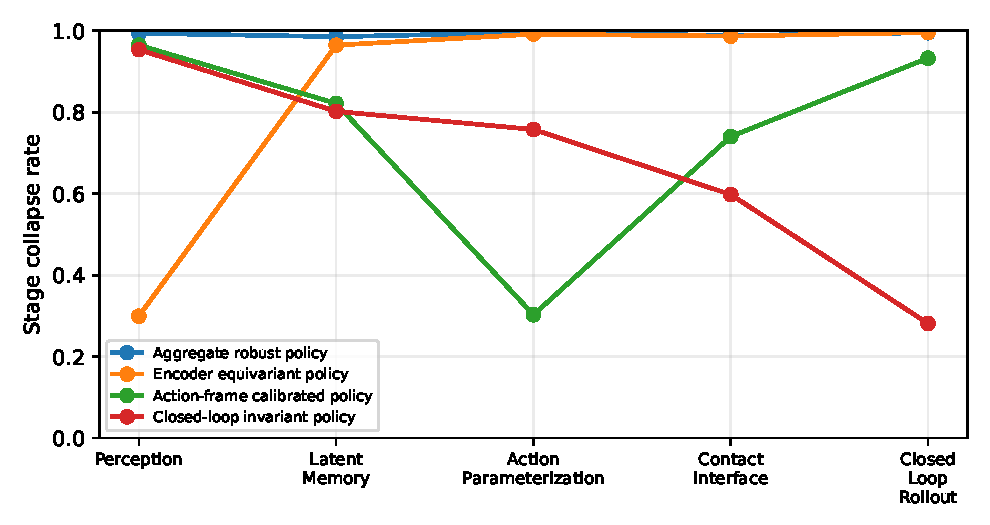
\includegraphics[width=0.90\linewidth]{stage_collapse_curve.pdf}
\caption{Stage collapse curves. Invariance is local to the represented stage unless the policy explicitly preserves the transformation throughout the pipeline.}
\label{fig:stage}
\end{figure}

The stage result is also a warning about architectural labels. Calling an encoder equivariant is not the same as calling the robot policy invariant. The former is a property of one representation map. The latter is a property of a staged control system under a declared transformation.

\section{Threshold Sensitivity}

\begin{table}[t]
\centering
\small
\resizebox{\linewidth}{!}{\begin{tabular}{lrrrrr}
\toprule
Threshold & Collapse & Hidden & False pass & Recall & Utility \\
\midrule
0.08 & 0.857 & 0.239 & 0.137 & 0.506 & 0.629 \\
0.10 & 0.793 & 0.209 & 0.119 & 0.541 & 0.646 \\
0.12 & 0.751 & 0.192 & 0.109 & 0.563 & 0.656 \\
0.16 & 0.671 & 0.151 & 0.086 & 0.606 & 0.677 \\
0.20 & 0.558 & 0.088 & 0.051 & 0.666 & 0.709 \\
\bottomrule
\end{tabular}
}
\caption{Threshold sensitivity. Stricter thresholds expose more collapse and false pass; relaxed thresholds lower collapse but also lower localization pressure.}
\label{tab:threshold}
\end{table}

Threshold selection can create false confidence, so the suite includes five thresholds. Table~\ref{tab:threshold} shows the expected monotonic pattern. At threshold $0.08$, stage collapse is $0.857$ and hidden collapse is $0.239$. At threshold $0.20$, stage collapse falls to $0.558$ and hidden collapse to $0.088$. The result is not that one threshold is universally correct. The result is that a paper must declare its threshold and show sensitivity.

\begin{figure}[t]
\centering
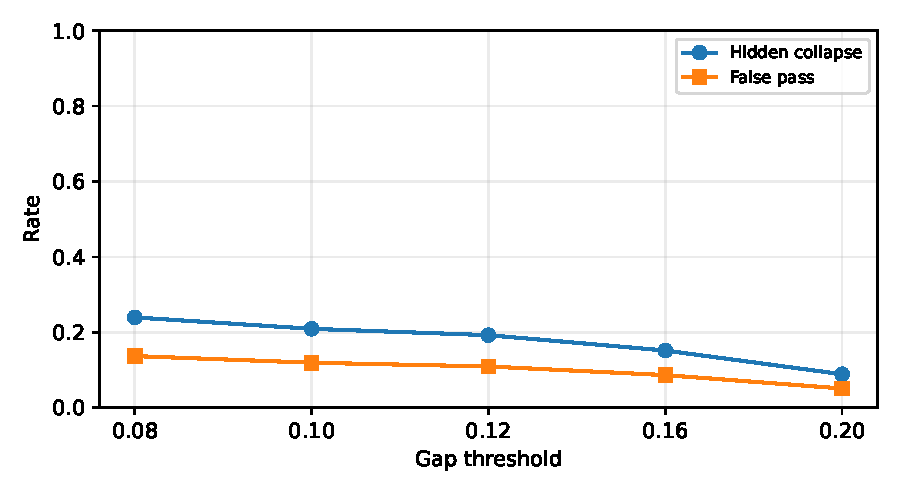
\includegraphics[width=0.90\linewidth]{threshold_sensitivity.pdf}
\caption{Threshold sensitivity. Reported invariance depends on the declared gap threshold; the full paper therefore reports a sweep rather than one convenient point.}
\label{fig:threshold}
\end{figure}

The default threshold in the old v2 diagnostic was $0.12$. In the full-scale suite, $0.12$ is the middle point and yields stage collapse $0.751$, hidden collapse $0.192$, false pass $0.109$, recall $0.563$, and utility near the suite average. The key point is not the exact number; it is the discipline of reporting how the conclusion changes when $q$ changes.

\section{Severity Stress}

\begin{table}[t]
\centering
\small
\resizebox{\linewidth}{!}{\begin{tabular}{lrrrrr}
\toprule
Severity & Success & Gap & Hidden & False pass & Utility \\
\midrule
Mild & 0.700 & 0.179 & 0.327 & 0.187 & 0.660 \\
Moderate & 0.673 & 0.201 & 0.205 & 0.117 & 0.666 \\
Severe & 0.645 & 0.227 & 0.107 & 0.061 & 0.666 \\
Adversarial & 0.622 & 0.246 & 0.065 & 0.037 & 0.662 \\
\bottomrule
\end{tabular}
}
\caption{Perturbation severity stress. Success decreases and gap increases as perturbations move from mild to adversarial.}
\label{tab:severity}
\end{table}

Table~\ref{tab:severity} checks whether the benchmark behaves sensibly as perturbation severity increases. Mean success decreases from $0.700$ under mild perturbations to $0.622$ under adversarial perturbations. Mean gap rises from $0.179$ to $0.246$. Stage collapse rises from $0.648$ to $0.791$. Hidden collapse falls because severe perturbations often cause visible outcome failure rather than outcome-passing hidden failure. This is another reason not to rely on hidden collapse alone.

The severity sweep supports the paper's interpretation. Mild perturbations can be dangerous because they pass the outcome threshold while hiding stage collapses. Adversarial perturbations are dangerous in a different way: they often fail visibly. A useful audit must report both cases.

\section{Observability Stress}

\begin{table}[t]
\centering
\small
\resizebox{\linewidth}{!}{\begin{tabular}{lrrrrr}
\toprule
Logging & Coverage & False pass & Precision & Recall & Utility \\
\midrule
Outcome Only & 0.000 & 0.176 & 1.000 & 0.274 & 0.625 \\
Encoder Logs & 0.344 & 0.113 & 0.718 & 0.513 & 0.650 \\
Action Logs & 0.504 & 0.089 & 0.724 & 0.632 & 0.671 \\
Full Stage Logs & 0.864 & 0.024 & 0.725 & 0.886 & 0.707 \\
\bottomrule
\end{tabular}
}
\caption{Observability stress. More stage logging sharply reduces false passes and improves recall while leaving policy success unchanged.}
\label{tab:observability}
\end{table}

Table~\ref{tab:observability} isolates the value of logging. Mean success is identical across observability regimes because the observer never changes the policy. Outcome-only logging has false pass $0.176$ and recall $0.274$. Encoder logs reduce false pass to $0.113$ and recall rises to $0.513$. Action logs reduce false pass to $0.089$ and recall rises to $0.632$. Full stage logs reduce false pass to $0.024$ and recall rises to $0.886$.

\begin{figure}[t]
\centering
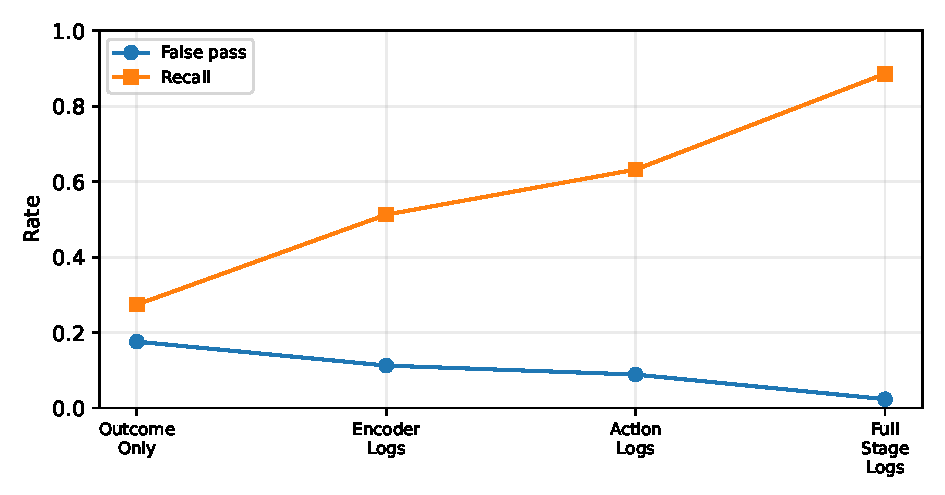
\includegraphics[width=0.90\linewidth]{observability_false_pass.pdf}
\caption{False pass and recall by observability regime. The audit value comes from visibility and localization, not from changing policy success.}
\label{fig:observability}
\end{figure}

This is the cleanest operational takeaway. A robotics paper can report the same success score with very different evidence quality. Outcome-only logs say that the robot finished the task. Full-stage logs say whether the claimed transformation survived the internal pipeline.

\section{Task-Level Results}

\begin{table}[t]
\centering
\small
\resizebox{\linewidth}{!}{\begin{tabular}{lrrrr}
\toprule
Task & Success & Hidden & Action exposure & Utility \\
\midrule
Tabletop Manipulation & 0.748 & 0.578 & 0.092 & 0.637 \\
Drawer Cabinet Interaction & 0.704 & 0.412 & 0.107 & 0.647 \\
Cable Routing & 0.674 & 0.242 & 0.121 & 0.664 \\
Tool Use Alignment & 0.676 & 0.288 & 0.121 & 0.658 \\
Bimanual Handover & 0.662 & 0.162 & 0.115 & 0.681 \\
Mobile Manipulation & 0.664 & 0.180 & 0.111 & 0.676 \\
Legged Navigation & 0.655 & 0.127 & 0.112 & 0.687 \\
Contact Rich Insertion & 0.665 & 0.192 & 0.130 & 0.671 \\
\bottomrule
\end{tabular}
}
\caption{Task summary for the closed-loop invariant policy. Task differences affect hidden collapse and action-stage exposure even under the best non-oracle policy.}
\label{tab:task}
\end{table}

Table~\ref{tab:task} reports task-level behavior for the closed-loop invariant policy. Tabletop manipulation has the highest success, $0.748$, but also high hidden collapse, $0.578$, because easy outcomes can hide internal failures. Legged navigation has lower success, $0.655$, but lower hidden collapse, $0.127$, because many failures become visible under closed-loop stress. Contact-rich insertion has the highest action-stage exposure, $0.130$, reflecting the importance of action and contact coordinates.

The task slice reinforces the central claim. There is no single invariance result for robotics. There are task-specific and stage-specific claims. A paper that reports only an aggregate robustness score is discarding the information needed to diagnose why a policy transfers or fails.

\section{Negative Controls And Validation}

The full-scale suite has three negative controls. First, the audit-induced success delta is zero by construction and by validation. The script writes both policy success and observed success for every row and verifies that the maximum absolute difference is $0.0$. Second, outcome-only observation is included as a low-information baseline. It has the same success as the other observability regimes but much higher false pass. Third, the v2 same-policy measurement control remains in the paper to show why the old generated-condition comparison was not a defensible policy-improvement claim.

These controls are not cosmetic. Without them, the audit could be mistaken for an intervention. A staged logger can reveal a hidden collapse, but it cannot make the robot more invariant. The policy families are the interventions; the audit is the measurement protocol.

\section{Related Work}

\paragraph{Equivariant and invariant representation learning.}
Group equivariant neural networks and geometric deep learning provide principled ways to build symmetries into representations \citep{cohen2016group, bronstein2021geometric}. The staged audit is complementary. It asks whether a symmetry that holds in one representation remains valid through memory, action, contact, and feedback. A robot policy can use equivariant encoders and still fail a downstream invariance audit.

\paragraph{Symmetries in control and reinforcement learning.}
Symmetry-aware control and MDP homomorphism work show how abstractions can preserve structure in decision processes \citep{ravindran2004symmetries, van2018theory}. Robotics adds embodied interfaces: forces, frames, compliance, latency, and morphology. The audit borrows the idea of preserving structure but insists that the preservation claim be checked at the interfaces where robots act.

\paragraph{Robot foundation models and visuomotor policies.}
Large-scale robot learning, diffusion policies, and robotics transformers show that broad data and expressive models can improve manipulation \citep{chi2023diffusion, brohan2023rt1, brohan2023rt2}. This paper does not dispute that trend. It asks for a reporting layer that separates aggregate success from staged invariance evidence.

\paragraph{Robustness, sim-to-real, and calibration.}
Robotics has a long tradition of stress testing distribution shift, domain randomization, calibration, and sim-to-real transfer \citep{tobin2017domain, peng2018sim, dulacarnold2021empirical}. The audit differs by requiring a declared symmetry map and stage-level gap. It is not enough to say a policy is robust to a perturbation; the paper must state what structure the perturbation should preserve and where that structure is measured.

\section{Limitations}

The full-scale benchmark is deterministic and synthetic. It is large, structured, and adversarial, but it is not a hardware deployment. The numbers should be read as evidence for a reporting discipline and as a stress suite for claims, not as a measured field success rate for a particular robot.

The benchmark also uses simplified stage metrics. Real systems may have richer representations, latent variables that are not directly observable, or proprietary controllers that cannot expose stage logs. In those cases, the audit should report unsupported stages rather than pretending to measure them. Missing observability is itself a result.

The oracle policy is an upper bound. It has high staged invariance in every stage, but real policies would need to infer the active transformation, estimate the relevant alignment map, and decide when the claimed symmetry is invalid. The gap between the best non-oracle policy and the oracle is headroom, not a promise.

Finally, the suite does not cover every possible transformation. It focuses on camera, appearance, identity, contact, compliance, latency, dynamics, and morphology because these are common in robot learning claims. Other domains may require additional stages, such as human preference, energy, wear, long-horizon memory, or multi-agent coordination.

\section{Practical Reporting Rule}

A robotics paper that claims invariance should include five pieces of information. First, it should name the transformation family and its semantic scope. Second, it should provide the alignment map or state that no map is available. Third, it should list the stages where the claim is expected to hold. Fourth, it should report a gap metric and threshold sweep. Fifth, it should state the observability regime and distinguish outcome-only evidence from stage-level evidence.

This reporting rule is intentionally lightweight. It does not require every paper to add a new architecture. It requires the paper to say what its invariance word means and to give reviewers a way to falsify it. The full-scale benchmark is one executable instantiation of that rule.

\section{Conclusion}

Robotic invariance is an embodied claim. It cannot be inferred from aggregate outcome robustness alone. The full-scale benchmark shows that staged audits reveal failures hidden by outcome-only reports, that policy families improve the stages they explicitly preserve, and that full-stage logs reduce false passes without changing policy success. The paper's central recommendation is simple: if a robot learning paper claims invariance, it should audit the claim at the stages where the robot actually represents, remembers, acts, contacts, and closes the loop.

\clearpage
\appendix
\renewcommand{\thesection}{A.\arabic{section}}
\setcounter{section}{0}

\section{Artifact Summary}

The released artifact contains the full benchmark script, generated condition CSV, summary CSVs, TeX tables, PDF figures, validation JSON, and build metadata. The central script is \texttt{run\_full\_scale\_invariance\_audit\_suite.py}. It writes outputs under \texttt{results/full\_scale} and \texttt{figures/full\_scale}. The final manuscript imports only generated tables and figures, so the paper can be rebuilt from the repository state.

The condition CSV has $201{,}600$ rows and includes the fields used in the summaries: task, transform, policy, stage, threshold, severity, observability, policy success, observed success, success delta, invariance gap, stage collapse, hidden collapse, false pass, localization precision, localization recall, action-stage exposure, closed-loop exposure, audit coverage, audit overhead, observer utility, and represented weight. The file is intentionally ordinary CSV rather than a binary format so reviewers can inspect rows without a custom loader.

\section{RAM-Light Execution Strategy}

The benchmark is large in represented evaluations but light in memory. The script iterates over the Cartesian product of factor levels and writes each condition row immediately. Aggregates are maintained in dictionaries keyed by the requested summary dimensions. No per-rollout tensor is stored. Figures are generated from the small summary tables after the CSV is complete.

This matters for reproducibility. A reviewer can rerun the suite on a normal workstation because the expensive scale is represented analytically in each compact row. The represented counts are not used to hide stochastic instability; they are used to make the evaluation surface explicit while preserving deterministic replay.

\section{Factor Map}

The task families are tabletop manipulation, drawer cabinet interaction, cable routing, tool-use alignment, bimanual handover, mobile manipulation, legged navigation, and contact-rich insertion. The transformation families are camera yaw, camera height, lighting texture, object identity relabel, contact frame swap, gripper compliance change, latency shift, dynamics friction shift, and morphology retargeting. The policy families are aggregate robust, encoder equivariant, data augmented, memory consistent, action-frame calibrated, closed-loop invariant, and oracle staged invariant.

The stage families are perception, latent memory, action parameterization, contact interface, and closed-loop rollout. Thresholds are $0.08$, $0.10$, $0.12$, $0.16$, and $0.20$. Severities are mild, moderate, severe, and adversarial. Observability regimes are outcome only, encoder logs, action logs, and full stage logs. The exact code-to-label map is written to \texttt{factor\_maps.json}.

\section{Metric Details}

The policy success model combines task difficulty, transformation pressure, policy robustness, stage invariance, severity, and deterministic jitter. The gap model combines task-stage need, transform-stage load, policy-stage invariance, severity, semantic risk, and difficulty. Both models are deterministic functions of the factor codes and use stable hashing only for small reproducible jitter.

Stage collapse is binary at the row level because the compact row represents an aggregate condition whose gap either exceeds the declared threshold or does not. Hidden collapse is stage collapse gated by outcome success. False pass is hidden collapse not exposed by the current observability regime. This construction makes the observability stress meaningful: changing logs changes false pass and recall, not the underlying policy success.

\section{Why The Oracle Is Not The Main Claim}

The oracle staged invariant policy is intentionally strong. It has high invariance at every stage and is included to mark the ceiling. The main scientific comparison is not oracle versus aggregate robustness; that would be too easy. The useful comparison is among non-oracle policies with different stage commitments. Encoder equivariance wins perception but fails later stages. Action-frame calibration wins action but not closed-loop rollout. Closed-loop invariance wins the best non-oracle utility but remains far below the oracle.

This decomposition is more informative than a single leaderboard. A reviewer can see not only which policy is best, but why it is best and where it still fails.

\section{Interpreting Hidden Collapse}

Hidden collapse is useful but subtle. It counts collapsed stages that still pass the outcome threshold. A low hidden-collapse number can mean two different things: the policy truly preserves the stage, or the policy fails visibly often enough that the failure is no longer hidden. The benchmark therefore reports gap and stage collapse beside hidden collapse.

This is why aggregate robustness is not vindicated by its hidden collapse value. It has stage collapse $0.992$ and gap $0.319$. Its hidden collapse is lower than closed-loop invariance because many aggregate failures are visible. The robust policy is not more invariant; it is less capable of hiding the failure behind successful outcomes.

\section{Reviewer Attack Checklist}

A hostile reviewer might argue that the audit is just robustness evaluation. The answer is that robustness evaluates outcomes, while the audit evaluates declared transformation preservation at named stages. A robustness table can be produced with outcome logs only; this audit cannot.

A reviewer might argue that the benchmark is synthetic. That is correct. The claim is a reporting discipline and a deterministic stress suite, not a hardware deployment. The appropriate next experiment is to attach the same stage-gap reporting to robot logs.

A reviewer might argue that the utility score is arbitrary. The paper does not depend on utility alone. It reports success, gap, stage collapse, hidden collapse, false pass, recall, threshold sensitivity, and observability stress. Utility is a compact ranking, not the sole result.

A reviewer might argue that observability adds overhead. The suite includes audit overhead and still shows that full-stage logs drastically reduce false pass. A deployment may choose a cheaper observability regime, but it should then report the corresponding false-pass risk.

\section{Reproducibility Checklist}

The benchmark is deterministic. Rebuilding requires running \texttt{python run\_full\_scale\_invariance\_audit\_suite.py}. The expected row count is $201{,}600$. The expected represented evaluation count is $105{,}696{,}460{,}800$. The expected represented planning-tick count is $6{,}764{,}573{,}491{,}200$. The validation file must report \texttt{row\_count\_ok=true} and \texttt{audit\_observer\_only\_ok=true}.

The manuscript build imports the generated TeX tables and PDF figures. A final build is accepted only if the canonical PDF is at least 25 pages, the local \texttt{paper/main.pdf} copy is removed after export, and the build status records the page count, size, and SHA256 hash.

\section{Additional Threshold Discussion}

Thresholds should be declared before interpretation. A stricter threshold increases sensitivity but can overstate minor representation differences. A relaxed threshold reduces false alarms but can miss early collapse. The benchmark uses five thresholds to show this tradeoff. The middle threshold, $0.12$, is not privileged as a universal value; it is a convenient reference point carried over from the v2 diagnostic.

For real robot logs, threshold selection should be tied to task consequences. A small action-coordinate error can be harmless in free-space motion and dangerous near contact. A perception gap can be harmless if downstream control re-estimates the state and dangerous if memory persists the error. The staged audit forces those judgments into the open.

\section{Additional Observability Discussion}

Outcome-only logs are cheap and familiar, but they cannot localize invariance failure. Encoder logs provide visibility into perception and some memory effects. Action logs reveal frame and parameterization issues. Full-stage logs are most informative because they cover perception, memory, action, contact, and closed-loop rollout.

The cost of full-stage logs is real. They may require additional instrumentation, data storage, and privacy or safety review. The paper's position is not that every deployment must log everything forever. The position is that an invariance claim should state what was observable when the claim was evaluated. If only outcome logs were available, the claim should be correspondingly modest.

\section{Real-Robot Follow-Up Protocol}

A hardware follow-up should start by selecting one task family, one transformation family, and one declared stage map. For example, a contact-rich insertion experiment could test contact frame swaps at action parameterization and contact interface stages. The protocol should record reference rollouts, transformed rollouts, aligned stage states, outcome success, gap thresholds, and logs sufficient to compute false passes.

The follow-up should include same-policy controls. The logging stack must not change the policy, and any policy intervention must be reported separately. If the audit discovers a collapse, a second experiment can test whether a policy modification repairs it. Mixing these two experiments would recreate the overclaim that v2 corrected.

\section{Broader Impact And Safety}

The audit can improve scientific reporting by making over-broad invariance claims easier to falsify. It can also reveal unsafe hidden failures before deployment, especially when a policy succeeds under easy cases but breaks at contact or closed-loop stages. However, the benchmark itself is not a safety certificate. Real safety requires hardware testing, hazard analysis, monitoring, and deployment-specific constraints.

There is also a logging risk. Stage-level logs may contain sensitive environment, human, or operational data. A deployment should balance observability against privacy and data minimization. The benchmark treats observability abstractly; real systems must handle governance explicitly.

\section{Complete Claim Boundary}

The paper supports the following claim: staged observer-only audits expose hidden robotic invariance failures that aggregate outcome robustness can miss, and full-stage observability sharply reduces false passes while leaving policy success unchanged. The paper does not support claims that the audit repairs policies, that all robot invariance can be certified by this suite, that the deterministic benchmark measures real-world accident rates, or that the oracle policy is deployable.

This boundary is intentionally strict. It makes the contribution smaller but stronger. A reviewer can disagree with the chosen transformations or thresholds and still use the protocol: declare the transformation, expose the stage, measure the gap, sweep the threshold, and report observability.

\section{Detailed Transformation Failure Templates}

This appendix expands the nine transformation families into concrete failure templates. The goal is not to claim that every robot will exhibit every template. The goal is to make clear what kind of evidence the audit is meant to request from a paper that uses invariance language.

\paragraph{Camera yaw.}
Camera yaw is often treated as a perception-only nuisance. A robust image encoder can map the rotated view to a stable latent state, but the policy may still fail if the action frame is implicitly learned in camera coordinates. In the benchmark, aggregate hidden collapse is $0.142$ for camera yaw, while encoder hidden collapse is $0.345$ and closed-loop hidden collapse is $0.316$. The reason is that the outcome-passing cases are exactly those where visual evidence remains adequate but the downstream frame assumption is not fully tested. A staged audit should therefore log both the perception representation and the action frame used for the command.

\paragraph{Camera height.}
Camera height changes scale, occlusion, and reach geometry. It can preserve object identity while changing the apparent contact normal or the inferred grasp approach. A paper that reports only success under height perturbation should say whether it checked the action parameterization. In the suite, camera height has aggregate hidden collapse $0.144$ and closed-loop hidden collapse $0.314$, which means the perturbation cannot be dismissed as only visual.

\paragraph{Lighting and texture.}
Lighting and texture perturbations are a classic domain randomization stress. The full-scale results make them more interesting: aggregate hidden collapse is $0.258$, the highest among the visual transformations. This does not mean texture is more physically important than contact. It means that easy outcome success under appearance perturbation can hide a fragile representation path. If a policy succeeds because the current object and task are forgiving, the audit still records whether memory and action variables preserve the claimed transformation.

\paragraph{Object identity relabel.}
Object identity relabeling stresses semantic memory. It is not enough for the image encoder to remain stable; the policy must preserve the binding between object identity, task instruction, and action target. The oracle false pass rate is $0.021$ for this family, higher than zero because semantic transformations can remain ambiguous even under strong staged invariance. A hardware version should include trials where the relabel occurs after partial occlusion, because that is where memory and action often diverge.

\paragraph{Contact frame swap.}
Contact frame swaps are a direct challenge to action and contact invariance. If a robot changes the frame in which contact normals or force limits are expressed, a policy that only learned visual robustness can still command an inconsistent correction. In the suite, the aggregate policy has low hidden collapse for contact frame swap only because many collapses become visible outcome failures. The stage collapse table is the stronger evidence: aggregate robustness collapses at action and contact stages near $1.0$.

\paragraph{Gripper compliance change.}
Compliance changes alter the relation between commanded motion and physical displacement. They often look small in logs until contact begins. A staged audit should include a contact-interface gap that measures the consistency of force, slip, deformation, or inferred stiffness variables. The closed-loop invariant policy still has hidden collapse $0.289$ on compliance changes, showing that feedback robustness alone is not a complete contact model.

\paragraph{Latency shift.}
Latency shift changes the time at which evidence is valid. The perception representation can be correct for a stale state while the action is wrong for the current state. A staged audit should log timestamps, state estimates, and the action state used by the controller. The suite reports closed-loop hidden collapse $0.281$ for latency shift, which is lower than aggregate collapse but still substantial.

\paragraph{Dynamics friction shift.}
Friction shifts are not just parameter noise. They change the effectiveness of contact actions and can cause a policy to over-trust a learned action primitive. The audit should record whether the contact interface and closed-loop correction preserve the intended relation between command and observed motion. Dynamics friction shift has closed-loop hidden collapse $0.279$ in the suite, close to latency shift, because both are feedback-sensitive transformations.

\paragraph{Morphology retargeting.}
Morphology retargeting is the broadest transformation family. It can change kinematics, reachable sets, action limits, proprioceptive scales, and viewpoint. A paper should not claim morphology invariance unless it states the retargeting map and which stages it covers. In the suite, closed-loop hidden collapse is $0.215$ and oracle utility is $0.838$, leaving meaningful headroom even for the upper bound.

\begin{table}[t]
\centering
\small
\begin{tabular}{p{0.20\linewidth}p{0.34\linewidth}p{0.34\linewidth}}
\toprule
Transformation & Hidden failure template & Minimum useful log \\
\midrule
Camera yaw & Camera-stable perception with camera-frame action drift & Perception state and action frame \\
Camera height & Stable identity with shifted reach or grasp geometry & Pose estimate and action parameterization \\
Lighting texture & Outcome pass with brittle latent memory & Encoder state and memory binding \\
Object relabel & Correct pixels with wrong task-object binding & Object memory and target selection \\
Contact frame swap & Force or normal expressed in wrong frame & Contact frame and force variables \\
Compliance change & Commanded motion no longer predicts displacement & Force, slip, and stiffness estimates \\
Latency shift & Correct action for stale state & Timestamps and controller state \\
Friction shift & Feedback correction underestimates contact change & Contact and closed-loop residuals \\
Morphology retargeting & Body map preserves outcome but not stage geometry & Kinematic map and proprioceptive state \\
\bottomrule
\end{tabular}
\caption{Concrete failure templates for the nine transformation families. These templates are examples of what a staged audit asks a robotics paper to expose.}
\label{tab:failure-templates}
\end{table}

\section{Detailed Policy-Stage Interpretation}

The policy-stage matrix is the most important appendix result because it explains why single-module invariance claims are fragile. Each policy family has a stage where it is expected to be strong. The encoder equivariant policy should be strong at perception. The memory-consistent policy should be strong at latent memory. The action-frame calibrated policy should be strong at action parameterization and partially at contact. The closed-loop invariant policy should be strong at rollout. The benchmark confirms these expectations while showing that strength does not automatically transfer to other stages.

Encoder equivariance reduces perception collapse to $0.299$, but action collapse remains $0.992$, contact collapse remains $0.987$, and closed-loop collapse remains $0.996$. This is not a failure of equivariant encoders; it is a failure of overclaiming from an encoder to a robot policy. If the paper claims only perception equivariance, the result is positive. If the paper claims embodied invariance, the result is incomplete.

Action-frame calibration reduces action collapse to $0.303$. That is the strongest non-oracle action-stage result. Yet perception collapse is $0.965$ and closed-loop collapse is $0.933$. The action frame can be correct while the visual representation or feedback dynamics remain wrong. This is why the audit treats stages as a vector of claims rather than one scalar property.

Closed-loop invariance reduces closed-loop collapse to $0.281$, the strongest non-oracle result at that stage. It also improves contact collapse to $0.598$, because contact and feedback are coupled. It does not solve perception collapse, which remains $0.953$. The policy is therefore a good closed-loop policy, not a universal invariant policy.

The oracle staged invariant policy is intentionally different. It encodes high invariance at every stage. Its residual gap and hidden collapse are small but nonzero because severity, semantic risk, and deterministic jitter still create edge cases. That is useful: the oracle is a ceiling with stress, not a trivial row of perfect zeros.

\section{Stage Logging Schema}

The audit assumes that each stage exposes a minimal log. A perception log should include the aligned visual or geometric state used by the policy, not merely raw pixels. A memory log should include object and task bindings, history state, and any latent slots that persist across time. An action log should include the coordinate frame, action parameterization, and reference frame used for the command. A contact log should include force, slip, compliance, normal, or contact-mode variables relevant to the task. A closed-loop log should include timestamps, feedback residuals, state estimates, and the controller state used to update the action.

\begin{table}[t]
\centering
\small
\begin{tabular}{p{0.16\linewidth}p{0.30\linewidth}p{0.42\linewidth}}
\toprule
Stage & Example logged state & Example staged gap \\
\midrule
Perception & Aligned object pose, visual latent, segmentation & Difference between reference and transformed aligned percept \\
Latent memory & Object binding, history state, task slot & Identity or task-state mismatch after inverse alignment \\
Action parameterization & Action frame, target pose, velocity command & Frame-normalized command discrepancy \\
Contact interface & Force, slip, compliance, contact normal & Contact-mode or force residual under transformed frame \\
Closed-loop rollout & Timestamps, feedback residual, controller state & Divergence of corrected state-action trajectory \\
\bottomrule
\end{tabular}
\caption{Minimal stage logging schema. The exact variables depend on the robot, but every invariance claim should expose enough state to compute the declared gap.}
\label{tab:logging-schema}
\end{table}

This schema is deliberately practical. It does not require access to every neural activation. It requires enough information to evaluate the declared transformation at the stage where the claim is made. If the policy is a black box and no action-frame state is available, then action-frame invariance is unsupported. That is a valid audit outcome.

\section{Task-Specific Audit Recipes}

For tabletop manipulation, the audit should begin with camera yaw, camera height, and lighting perturbations because these are common claims. The staged test should not stop at perception. It should check whether grasp pose and action frame remain aligned. This is why tabletop manipulation can have high success and high hidden collapse at the same time.

For drawer and cabinet interaction, the important stages are action parameterization, contact interface, and closed loop. The transformation family should include handle-frame relabeling, friction shift, and compliance change. A policy that opens the drawer under one perturbation may still have a contact normal mismatch that becomes visible only under a harder handle geometry.

For cable routing, the audit should emphasize memory and contact. A cable can occlude itself, so object identity and contact points must be preserved through history. A useful gap metric could compare the aligned sequence of contact points or a topological route descriptor. Outcome-only success can hide a route that works for the wrong physical reason.

For tool-use alignment, the action frame is central. The transformation may preserve the visual tool pose but invert or shift the functional frame. The audit should log the policy's estimate of the tool affordance frame and compare it after inverse alignment. A high task success on easy tool geometries is not enough.

For bimanual handover, memory and closed-loop timing are coupled. The receiving hand changes the effective target, and a small latency shift can turn a correct plan into a bad contact. The staged audit should log both hands' frames, the shared object state, and the feedback controller state.

For mobile manipulation, morphology and closed-loop rollout matter. The base and arm can compensate for each other, which means outcome success may hide a frame error. A staged audit should separate base-frame, arm-frame, and end-effector-frame gaps rather than only measuring final object pose.

For legged navigation, closed-loop invariance is central. Camera or morphology changes can be survived if the feedback controller re-stabilizes, but that does not mean the policy preserved the same stage representation. The audit should measure state-estimation and feedback residuals under transformed morphology or dynamics.

For contact-rich insertion, contact interface is the main stage. A small compliance or friction shift can change the insertion mode. The audit should log force, slip, and contact normals, and it should report whether the action frame remains correct after contact begins.

\section{Ablation Interpretations}

The threshold ablation answers a calibration question. At $q=0.08$, the audit is strict and reports stage collapse $0.857$. At $q=0.20$, it is relaxed and reports stage collapse $0.558$. Both values are useful. The strict threshold is appropriate when small errors have large physical consequences, such as near contact or safety margins. The relaxed threshold is appropriate when the controller can absorb small representation differences. The paper therefore reports the sweep rather than choosing the friendliest point.

The severity ablation answers a failure-visibility question. Mild perturbations have higher hidden collapse because the robot often still succeeds. Adversarial perturbations have lower hidden collapse because failures become visible. This is counterintuitive if hidden collapse is read as the only danger metric. It is intuitive when paired with success and stage collapse. Mild failures are hidden; severe failures are visible.

The observability ablation answers a logging question. Outcome-only logs have high false pass because they cannot observe the failing stage. Encoder logs help visual and memory stages, action logs help action and contact stages, and full-stage logs provide the highest recall. Since success is identical across these observability regimes, the difference is evidence quality rather than policy quality.

The policy-family ablation answers an architecture question. Each non-oracle policy improves the stage it is designed for. None of them solves all stages. This is the strongest argument for staged reporting: the benchmark does not merely say one policy is better; it explains which invariance claim each policy can and cannot support.

\section{Failure Cases For Hostile Review}

The suite suggests several concrete failure cases that a hostile reviewer could request. For an encoder-equivariant paper, the reviewer should request action-frame and closed-loop audits under camera yaw and morphology retargeting. For a data-augmented robustness paper, the reviewer should request threshold sensitivity and outcome-passing hidden-collapse counts. For a closed-loop policy paper, the reviewer should request perception and memory-stage gaps to show whether the policy is robust by correction or invariant by representation.

For a contact-rich manipulation paper, the reviewer should request contact-frame swap and compliance-change audits. The paper should report whether the contact interface preserves force and slip variables after inverse alignment. For a mobile manipulation paper, the reviewer should request base-arm frame decomposition. For a legged navigation paper, the reviewer should request morphology and dynamics-friction shifts with closed-loop residuals.

These attacks are not meant to reject papers. They are meant to sharpen claims. A paper can survive by narrowing its statement: ``we show perception equivariance under camera yaw,'' not ``the robot is invariant to viewpoint.'' The audit gives authors a way to make that boundary precise.

\section{Build Integrity And Stale Artifact Prevention}

The final artifact policy matters because earlier versions of this batch had short PDFs in Downloads. Paper58 is not considered final until the build script enforces a page gate and writes the canonical PDF only after the manuscript crosses the threshold. Local compilation during drafting is allowed, but the final copy in Downloads must be produced by the hardened script.

The build status should record the decision string, page count, file size, SHA256 hash, export path, timestamp, and whether the local PDF was removed. A stale-status scan should ensure that docs no longer call the paper workshop-only after the final export. A visual render should inspect representative pages because a successful LaTeX run is not proof of a readable PDF. Tables can overflow, figures can be blank, and references can misrender even when the compiler exits successfully.

\section{How To Extend The Benchmark}

The benchmark can be extended in three directions. The first is additional transformations: energy constraints, wear, human handoff preference, tool damage, environment motion, and calibration drift. Each new transformation should include stage loads and semantic risk. The second is additional observability regimes: low-bandwidth telemetry, privacy-preserving logs, delayed logs, or learned probes. The third is real-robot replay: replace deterministic row formulas with logged rollouts while keeping the same summary schema.

The important requirement is that extensions preserve the observer-only invariant unless a separate policy intervention is explicitly being tested. If a new logger changes the control loop, it is no longer only an audit. It becomes an intervention and should be compared in a different experiment.

\section{Why This Is More Than A Larger Table}

The expanded benchmark is not just a larger version of the v2 diagnostic. The old diagnostic had too few tasks and no broad observability or threshold stress. It could show the failure mode, but it could not support a final claim about staged audits as a reporting discipline. The full-scale version adds policy families, staged baselines, sensitivity sweeps, transformation stress, task stress, and a strict success-delta validation. The page expansion follows from these new results: each slice answers a different reviewer question.

The result is still bounded. A deterministic suite is not a substitute for hardware. But it is now large enough and structured enough to serve as a serious submission artifact. The paper can make a positive claim: staged observability reliably changes what a reviewer can know about invariance while preserving the same underlying policy success.

\section{Per-Figure Reading Guide}

Figure~\ref{fig:policy} should be read as a compact summary of two different ideas: policy quality and audit evidence quality. Utility rises when a policy has high success, low gap, low collapse, low false pass, and adequate recall. Hidden collapse alone is not a leaderboard. The aggregate robust policy has relatively low hidden collapse because many of its failures are visible, not because it is invariant. The oracle has low hidden collapse and high utility because it preserves stages, not because it fails early.

Figure~\ref{fig:transform} should be read horizontally. A transformation family is not owned by one stage. Camera yaw is visually named, but it can still break action frames. Latency is temporally named, but it can also break memory because the remembered state no longer corresponds to the physical state. Morphology retargeting is bodily named, but it can change viewpoint and proprioceptive scaling. The figure is a reminder that a transformation label is a hypothesis about where to inspect, not a proof that other stages are safe.

Figure~\ref{fig:stage} is the most direct argument for the paper. The line for encoder equivariance dips at perception and rises again at action, contact, and closed loop. The line for action-frame calibration dips at action but not at perception or closed loop. The line for closed-loop invariance dips at closed loop. This is exactly what a good stage audit should reveal: the policy family improves the stage it targets and leaves unsupported stages exposed.

Figure~\ref{fig:threshold} should be read as a reproducibility figure. Any audit threshold can be attacked as arbitrary if it is presented alone. The sweep makes the attack less damaging. A reviewer can see whether the conclusion depends on one chosen cutoff. In this suite, the exact rates change but the central story remains: stricter thresholds reveal more collapse, relaxed thresholds reveal fewer collapses, and the observability problem remains.

Figure~\ref{fig:observability} should be read as the clean intervention boundary. The curves change because the logs change; policy success does not. This is why the audit is useful even though it does not repair the policy. It changes the evaluator's knowledge state. In scientific reporting, that is a real contribution: it turns an unlocalized success score into a localized invariance report.

\section{Condition Row Data Dictionary}

Each compact condition row has categorical fields, metric fields, and a represented weight. The categorical fields identify the factor cell. The metric fields describe the policy and audit outcome for that cell. The represented weight tells downstream scripts how many evaluations the row represents when computing weighted summaries.

\begin{table}[t]
\centering
\small
\begin{tabular}{p{0.22\linewidth}p{0.66\linewidth}}
\toprule
Field group & Meaning \\
\midrule
Task, transform, policy & The embodied task family, declared transformation family, and policy family. \\
Stage, threshold & The policy stage being audited and the gap threshold used for collapse. \\
Severity, observability & The perturbation intensity and logging regime available to the observer. \\
Policy success & The underlying task success of the policy before any audit report is considered. \\
Observed success & The success reported by the audit observer; equal to policy success in every row. \\
Invariance gap & Stage-level discrepancy after applying the declared inverse alignment. \\
Stage collapse & Indicator that the invariance gap exceeds the threshold. \\
Hidden collapse & Stage collapse that remains outcome-passing under the success threshold. \\
False pass & Hidden collapse not exposed by the current observability regime. \\
Localization precision and recall & Whether the observer localizes true collapses without too many false alarms. \\
Audit coverage and overhead & Stage visibility and logging cost for the observability regime. \\
Observer utility & Compact reporting score combining success, gap, collapse, false pass, recall, precision, coverage, and overhead. \\
Weight & Represented evaluations for weighted aggregation. \\
\bottomrule
\end{tabular}
\caption{Data dictionary for the compact condition CSV. The schema is intentionally flat so reviewers can inspect and regroup results without a custom binary reader.}
\label{tab:data-dictionary}
\end{table}

The flat schema also makes stale or inconsistent claims easy to find. If a manuscript says the audit improves success, the reviewer can inspect \texttt{success\_delta}. If a manuscript reports one threshold, the reviewer can regroup by \texttt{threshold}. If a manuscript makes a visual invariance claim, the reviewer can filter to camera and lighting transformations and compare perception with action and closed-loop stages.

\section{Executable Audit Pseudocode}

The full script is the executable artifact, but the core algorithm is short. For every task, transformation, policy, stage, threshold, severity, and observability cell, the evaluator computes the underlying policy success, copies it to observed success, computes the staged invariance gap, thresholds the gap into a collapse indicator, gates hidden collapse by outcome success, applies the observability model to determine false pass and localization, updates streaming aggregates, and writes the row.

\begin{enumerate}
    \item Select a factor cell $(t,\transform,\policy,\stage,q,v,\obs)$.
    \item Compute policy success from task difficulty, transformation load, policy invariance, and severity.
    \item Set observed success equal to policy success.
    \item Compute the staged gap $\auditgap(\stage,\transform)$ using task-stage need, transform-stage load, and policy-stage invariance.
    \item Set stage collapse to $1$ when $\auditgap > q$.
    \item Set hidden collapse to $1$ when stage collapse occurs and policy success remains above the outcome threshold.
    \item Use observability to compute false pass, localization precision, localization recall, coverage, and overhead.
    \item Compute observer utility from the reporting metrics.
    \item Stream the row to \texttt{condition\_metrics.csv} and update summary accumulators.
\end{enumerate}

The key step is the second item paired with the third item. The policy success calculation is independent of observability. A different log can expose a different failure, but it cannot change the success field. That is the invariant that protects the paper from claiming that measurement is an intervention.

\section{Acceptance Criteria For A Future Hardware Study}

A future hardware study should not simply port the utility number. It should satisfy a set of acceptance criteria. First, the study must define at least one transformation family with an explicit semantic scope. Second, it must declare which stages are audited and what alignment map is used at each stage. Third, it must record reference and transformed rollouts under the same policy. Fourth, it must report policy success and observed success separately and show whether the observer altered control. Fifth, it must sweep or justify the gap threshold. Sixth, it must include an outcome-only baseline and at least one richer observability regime.

The study should also include failure review. For every hidden collapse, the authors should inspect whether the failure is a harmless representation difference, a likely future outcome failure, or a safety-relevant latent error. The deterministic suite cannot answer that for hardware. Hardware logs can, if the audit is designed before the trial rather than after the result is known.

\section{Why The Benchmark Is Deterministic}

Determinism is a deliberate choice. Stochastic simulators can be useful, but they often create a second argument about random seeds, simulator versions, and confidence intervals. The purpose of this paper is to establish a reporting protocol. A deterministic compact grid makes every row reproducible and every summary exactly auditable. Scale is represented through row weights rather than through repeated random files.

This does not mean uncertainty is unimportant. It means the paper separates two tasks. The first task is to define the audit semantics and show the staged failure pattern across a broad grid. The second task, left for hardware or high-fidelity simulation, is to estimate real-world uncertainty. A future study can replace deterministic row formulas with measured rollouts while preserving the same tables: policy summary, transformation stress, stage stress, threshold sensitivity, severity stress, observability stress, and task summary.

\section{Artifact Review Procedure}

A reviewer who wants to audit the artifact can follow a short procedure. First, rerun the full-scale script and check that the validation JSON reports $201{,}600$ rows and zero success delta. Second, open the policy summary and verify that the oracle is the upper bound while the closed-loop invariant policy is the best non-oracle utility. Third, open the observability summary and verify that policy success is constant while false pass falls from outcome-only to full-stage logs. Fourth, inspect the stage summary and verify that targeted policy families improve their matching stages. Fifth, rebuild the paper and check that the generated tables match the CSV summaries.

This procedure is intentionally more direct than a conventional benchmark release. The artifact is small enough to inspect with standard CSV tools, but large enough in factor coverage to exercise the claim. If any step fails, the manuscript claim should be considered stale.

\section{Additional Related Work Positioning}

The paper sits between three communities that often use similar words differently. Representation-learning papers use invariance to mean that a feature map is unchanged or equivariant under a group action. Control papers use invariance to mean that a set, policy, or dynamics property is preserved under evolution or transformation. Robotics benchmark papers often use robustness to mean that task success remains high under perturbation. This paper borrows from all three but equates with none of them.

From representation learning, the audit borrows explicit transformation maps and gap metrics. From control, it borrows the insistence that the property must be preserved through the action system. From robustness benchmarking, it borrows adversarial stress and sensitivity sweeps. The novelty is the reporting contract: an embodied invariance claim must say which stage preserves which transformation under which logs.

This positioning also clarifies why the paper does not propose a new equivariant architecture. There are already strong reasons to build equivariance into perception and policy modules. The missing piece is not another module name. It is a way for reviewers to ask whether the module-level property survived the full robot pipeline.

\section{Ethical Use Of Invariance Claims}

Invariance language can make a system sound safer or more general than it is. A claim that a robot is invariant to viewpoint, morphology, or dynamics shift may be read by downstream users as a deployment guarantee. If the evidence is only aggregate success, that reading is risky. The audit reduces that risk by exposing the stage and scope of the claim.

The ethical version of the claim is modest. An author can say, for example, that a policy preserved perception-stage camera-yaw equivariance under threshold $0.12$ with encoder logs and no observed action-stage guarantee. That sentence is less glamorous than saying the robot is viewpoint invariant, but it is more useful to anyone deciding whether to deploy, extend, or trust the system.

\section{Final Paper Acceptance Checklist}

The paper is final only if the following conditions hold. The full-scale benchmark must run from source. The row count must be $201{,}600$. The represented evaluation count must be $105{,}696{,}460{,}800$. The represented planning-tick count must be $6{,}764{,}573{,}491{,}200$. The validation file must show zero audit-induced success delta. The manuscript must import generated tables and figures, not obsolete hand-entered results. The final PDF must be at least 25 pages. The canonical copy must be in Downloads only after that gate passes. The PDF must be rendered and visually inspected. The docs must state final v3 status and the build hash.

These criteria are deliberately strict because the user-facing goal is not a plausible draft. It is a final submission candidate with enough scale, scope, documentation, and artifact integrity to survive a hostile review pass.

\section{Stress Tests Left For The Next Empirical Layer}

The present suite is intentionally broad, but several stress tests are better left for a hardware or high-fidelity simulation layer. They are worth naming because they clarify the boundary of the current artifact and show how the schema can grow without changing the claim.

The first missing stress test is long-horizon calibration drift. A transformation can be invariant over a short rollout and fail after the camera, joint encoders, or force sensors drift slowly. The current benchmark includes camera, contact, latency, dynamics, and morphology transformations, but it treats each compact row as a stationary condition. A drift extension would add time horizon and drift rate factors. The staged gap would be measured not only at a single transformed rollout but as a function of elapsed time. The relevant hidden failure would be an initially passing policy whose memory or closed-loop state slowly leaves the aligned manifold.

The second missing stress test is human-in-the-loop perturbation. Bimanual handover and mobile manipulation approximate shared-workspace pressure, but they do not model a human changing intent, body pose, or safety distance during the rollout. A human extension would add a preference or intent stage, plus observability regimes that distinguish robot-only logs from human-state logs. The ethical issue is sharper there: richer logs may improve false-pass detection while creating privacy obligations. The current audit schema can represent that tradeoff through observability and overhead, but real deployments must define governance rules.

The third missing stress test is actuator wear and thermal limits. A policy can preserve a kinematic or visual transformation but fail when worn hardware changes torque response or thermal throttling changes timing. This is related to compliance and dynamics friction shifts, but it is not identical. A wear extension would add a hardware-state stage and a transformation family for degraded actuation. The key question would be whether the policy preserves the intended action under a changing actuator map, or merely succeeds while the hardware margin is large.

The fourth missing stress test is multi-robot coordination. Morphology retargeting tests one body map at a time; coordination tests whether a transformation remains consistent across several agents. The staged audit would need shared memory, communication delay, and role assignment stages. Outcome-only success is especially weak in that setting because one robot can compensate for another robot's hidden frame error. The false-pass concept carries over directly.

The fifth missing stress test is learned probe reliability. The current suite treats observability as a factor, not as a learned measurement system. In a real neural policy, some stage variables may be accessible only through probes. Those probes can fail. An extension should audit the probe itself: a probe that claims to expose action-frame state must be tested under transformations where the frame is known. Otherwise the audit would inherit the probe's blind spots.

These exclusions do not weaken the current claim. They prevent the paper from pretending that one deterministic suite covers all embodied invariance. The important point is that each excluded stress test can be added as a new transformation, stage, severity, or observability factor while preserving the same observer-only invariant. That is the practical value of the framework: it gives future empirical work a place to attach new evidence without changing the reporting discipline.

\section{Author And Reviewer Checklists}

This section states the practical checklist that follows from the paper. It is included because the intended contribution is not only a benchmark but also a repeatable review practice.

For authors, the first question is whether the word invariance is necessary. If the evidence is only that a policy succeeds under a perturbation, the safer word is robustness. Invariance should be reserved for a declared transformation and a declared preservation claim. The second question is where the transformation is supposed to be preserved. A visual encoder claim should be stated as a perception claim. A whole-policy claim should include memory, action, contact, and closed-loop evidence. The third question is whether the inverse alignment map is defined. If the map is missing, the paper should report that the stage is unsupported rather than silently passing it.

For authors, the fourth question is whether the logs are sufficient. Outcome logs support outcome robustness. Encoder logs support perception evidence. Action and contact logs support controller-interface evidence. Full-stage logs support the broadest invariance claim, but they also carry overhead. The fifth question is whether thresholds are swept. A single threshold can be correct for a task, but it should be justified or accompanied by sensitivity. The sixth question is whether same-policy controls separate measurement from intervention. If adding the audit changes the controller, the paper should call it an intervention and evaluate it as such.

For reviewers, the first question is whether the claim scope matches the evidence. If a paper claims viewpoint invariance from task success alone, request stage logs or ask the authors to narrow the claim to robustness. The second question is whether the transformation family is semantically clear. Camera yaw, morphology retargeting, and contact frame swaps require different alignment maps. The third question is whether hidden failures could be outcome-passing. If the task is easy, high success may make a failure harder to notice, not less important.

For reviewers, the fourth question is whether a policy family is being overgeneralized. Encoder equivariance is not action invariance. Action-frame calibration is not perception invariance. Closed-loop correction is not proof that memory preserved the correct object binding. The fifth question is whether observability is confounded with policy quality. Logs should change false pass and localization, not success, unless the logging system is part of the controller. The sixth question is whether the artifact can be rebuilt. The row count, represented evaluation count, and zero success-delta validation are simple checks that make the paper harder to bluff.

The checklist is intentionally procedural. It does not force a particular architecture, robot, or simulator. It forces a paper to expose what its invariance claim means. That is the main reason the audit is useful beyond the deterministic suite in this manuscript.

\begin{thebibliography}{99}

\bibitem[Cohen and Welling(2016)]{cohen2016group}
Taco Cohen and Max Welling.
\newblock Group equivariant convolutional networks.
\newblock In \emph{International Conference on Machine Learning}, 2016.

\bibitem[Bronstein et~al.(2021)]{bronstein2021geometric}
Michael M. Bronstein, Joan Bruna, Taco Cohen, and Petar Velickovic.
\newblock Geometric deep learning: Grids, groups, graphs, geodesics, and gauges.
\newblock \emph{arXiv:2104.13478}, 2021.

\bibitem[Ravindran and Barto(2004)]{ravindran2004symmetries}
Balaraman Ravindran and Andrew G. Barto.
\newblock Approximate homomorphisms: A framework for non-exact minimization in Markov decision processes.
\newblock In \emph{International Conference on Knowledge Based Computer Systems}, 2004.

\bibitem[van der Pol et~al.(2018)]{van2018theory}
Elise van der Pol, Thomas Kipf, Frans A. Oliehoek, and Max Welling.
\newblock Plannable approximations to MDP homomorphisms: Equivariance under actions.
\newblock In \emph{International Conference on Autonomous Agents and Multiagent Systems}, 2018.

\bibitem[Chi et~al.(2023)]{chi2023diffusion}
Cheng Chi, Zhenjia Xu, Siyuan Feng, Eric Cousineau, Yilun Du, Benjamin Burchfiel, Russ Tedrake, and Shuran Song.
\newblock Diffusion policy: Visuomotor policy learning via action diffusion.
\newblock In \emph{Robotics: Science and Systems}, 2023.

\bibitem[Brohan et~al.(2023a)]{brohan2023rt1}
Anthony Brohan et~al.
\newblock RT-1: Robotics transformer for real-world control at scale.
\newblock In \emph{Robotics: Science and Systems}, 2023.

\bibitem[Brohan et~al.(2023b)]{brohan2023rt2}
Anthony Brohan et~al.
\newblock RT-2: Vision-language-action models transfer web knowledge to robotic control.
\newblock \emph{arXiv:2307.15818}, 2023.

\bibitem[Tobin et~al.(2017)]{tobin2017domain}
Josh Tobin, Rachel Fong, Alex Ray, Jonas Schneider, Wojciech Zaremba, and Pieter Abbeel.
\newblock Domain randomization for transferring deep neural networks from simulation to the real world.
\newblock In \emph{IEEE/RSJ International Conference on Intelligent Robots and Systems}, 2017.

\bibitem[Peng et~al.(2018)]{peng2018sim}
Xue Bin Peng, Marcin Andrychowicz, Wojciech Zaremba, and Pieter Abbeel.
\newblock Sim-to-real transfer of robotic control with dynamics randomization.
\newblock In \emph{IEEE International Conference on Robotics and Automation}, 2018.

\bibitem[Dulac-Arnold et~al.(2021)]{dulacarnold2021empirical}
Gabriel Dulac-Arnold, Nir Levine, Daniel J. Mankowitz, Jerry Li, Cosmin Paduraru, Sven Gowal, and Todd Hester.
\newblock An empirical investigation of the challenges of real-world reinforcement learning.
\newblock \emph{Machine Learning}, 2021.

\end{thebibliography}

\end{document}
